\chapter{Weber-Kraft}
\section{Die Gleichung der Weber-Elektrodynamik}
Die Weber-Elektrodynamik stellt eine alternative Formulierung der elektrodynamischen Wechselwirkungen dar, die auf einer Erweiterung des Coulombschen Gesetzes basiert (\refeq{eq:weber_em}).

Diese Gleichung beschreibt die Kraft zwischen zwei Ladungen $q_1$ und $q_2$, wobei $r$ der Abstand zwischen ihnen ist, $\dot{r}$ die relative Geschwindigkeit, $\ddot{r}$ die relative
Beschleunigung und $c$ die Lichtgeschwindigkeit. Der erste Term entspricht der klassischen Coulomb-Kraft, während die zusätzlichen Terme geschwindigkeits- und beschleunigungsabhängige
Effekte berücksichtigen.

\subsection{Impuls und Energie}
In der Weber-Elektrodynamik wird der Impuls- und Energietransport direkt durch die Wechselwirkung zwischen Ladungen beschrieben. Die Gesamtenergie des Systems setzt sich aus der potentiellen
Energie der Coulomb-Wechselwirkung und den kinetischen Termen der relativen Bewegung zusammen:

\[
    E = \frac{1}{2} m_1 v_1^2 + \frac{1}{2} m_2 v_2^2 + \frac{q_1 q_2}{4 \pi \epsilon_0 r} \left[ 1 - \frac{\dot{r}^2}{2c^2} \right]
\]

Diese Formulierung zeigt, wie die Weber-Theorie die Energieerhaltung auch bei dynamischen Prozessen gewährleistet.

\subsection{Lichtgeschwindigkeit und Raummodell}
Ein zentraler Aspekt der Weber-Elektrodynamik ist ihre Behandlung der Lichtgeschwindigkeit $c$. Im Gegensatz zur \gls{srt}, die $c$ als absolute Konstante postuliert,
erscheint $c$ in der Weber-Theorie als Parameter, der die Ausbreitungsgeschwindigkeit von Wechselwirkungen bestimmt. Dies ermöglicht ein Raummodell, in dem die Lichtgeschwindigkeit
nicht als universelle Grenze, sondern als Eigenschaft der Wechselwirkung selbst interpretiert wird.

\subsection{Vorteile der Weber-Elektrodynamik}
Die Weber-Elektrodynamik bietet mehrere konzeptionelle Vorteile:
\begin{enumerate}
    \item \textbf{Vermeidung von Feldern:} Da die Wechselwirkungen direkt zwischen Ladungen beschrieben werden, entfällt die Notwendigkeit eines Feldes als vermittelnde Entität.
    \item \textbf{Konsistente Fernwirkung:} Die Theorie vereint instantane und retardierte Effekte in einer einzigen Gleichung, wodurch die scheinbaren Widersprüche der klassischen Fernwirkung aufgelöst werden.
    \item \textbf{Energieerhaltung:} Die Weber-Kraft gewährleistet automatisch die Erhaltung von Energie und Impuls, ohne zusätzliche Annahmen.
    \item \textbf{Alternative Darstellung:} Die Theorie bietet eine Möglichkeit, elektrodynamische Phänomene ohne die Postulate der speziellen Relativitätstheorie zu beschreiben.
\end{enumerate}

Die Weber-Elektrodynamik stellt eine elegante und konsistente Alternative zur herkömmlichen Feldtheorie dar. Durch ihre Kombination aus instantanen und retardierten Effekten ermöglicht
sie ein tieferes Verständnis der elektrodynamischen Wechselwirkungen und eröffnet neue Perspektiven auf fundamentale Fragen der Physik, wie die Natur der Lichtgeschwindigkeit und die Struktur
des Raumes.

\section{Vergleichende Beispielrechnungen}
\subsection{Kraft zwischen gleichförmig bewegten Ladungen}

\textbf{Szenario:} Zwei Punktladungen $q_1 = q_2 = e$ (Elementarladung) bewegen sich parallel mit $v = 0,\!1c$ im Abstand $d = 1\,\text{\AA}$.

\begin{table}[ht]
\centering
\caption{Kraftberechnung im Vergleich}
\begin{tabular}{lcc}
\toprule
 & \textbf{Maxwell} & \textbf{Weber} \\
\midrule
Coulomb-Term & $\displaystyle\frac{e^2}{4\pi\epsilon_0 d^2}$ & $\displaystyle\frac{e^2}{4\pi\epsilon_0 d^2}\left(1-\frac{v^2}{c^2}\right)$ \\
Magnetischer Term & $\displaystyle\frac{\mu_0 e^2 v^2}{4\pi d^2}$ & -- \\
\hline
Kraftasymmetrie & $2F_B = 5,\!12\times10^{-11}\,\text{N}$ & $0$ \\
\bottomrule
\end{tabular}
\end{table}

\begin{equation}
F_{\text{Weber}} = \frac{e^2}{4\pi\epsilon_0 d^2}\left[1 - \frac{v^2}{c^2}\right] \approx 2,\!29\times10^{-8}\,\text{N}
\end{equation}

\subsection{Strahlungsdämpfung harmonischer Schwingung}

Für ein Elektron mit $x(t) = x_0\cos(\omega t)$:

\begin{align}
\textbf{Maxwell:}\quad & P = \frac{e^2\omega^4 x_0^2}{6\pi\epsilon_0 c^3}\cos^2(\omega t) \\
\textbf{Weber:}\quad & F_{\text{dampf}} = -\frac{e^2\omega^2\dot{x}}{4\pi\epsilon_0 c^3}
\end{align}

\begin{figure}[ht]
\centering
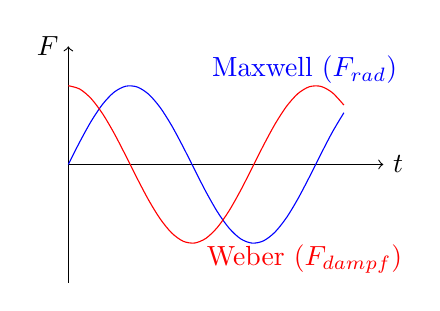
\begin{tikzpicture}
\draw[->] (0,0) -- (4,0) node[right]{$t$};
\draw[->] (0,-1.5) -- (0,1.5) node[left]{$F$};
\draw[domain=0:3.5,smooth,variable=\x,blue] plot ({\x},{sin(2*\x r)});
\draw[domain=0:3.5,smooth,variable=\x,red] plot ({\x},{cos(2*\x r)});
\node[blue] at (3,1.2) {Maxwell ($F_{\text{rad}}$)};
\node[red] at (3,-1.2) {Weber ($F_{\text{dampf}}$)};
\end{tikzpicture}
\caption{Zeitlicher Verlauf der Rückwirkungskräfte}
\end{figure}

\subsection{Interpretation der Ergebnisse}

\begin{itemize}
\item \textbf{Actio=Reactio:} Während die Maxwell-Theorie eine Asymmetrie von $2F_B$ zeigt, bleibt in der Weber-Elektrodynamik die Symmetrie gewahrt.

\item \textbf{Strahlungsdämpfung:} Die Weber-Theorie liefert eine lokale Beschreibung der Dämpfung ohne die kausalen Paradoxien der Abraham-Lorentz-Kraft:

\begin{equation}
\tau_{\text{Weber}} = \frac{e^2}{4\pi\epsilon_0 m c^3} \approx 6,\!3\times10^{-24}\,\text{s}
\end{equation}

\item \textbf{Energieerhaltung:} Beide Theorien erhalten die Gesamtenergie, aber die Weber-Elektrodynamik benötigt kein separates Feldkonzept.
\end{itemize}

\section{Vektorielle Form der Weber-Kraft}
\subsection{Herleitung aus der skalaren Form}

Die skalare Weber-Kraft (Gl.~\ref{eq:weber_scalar}):

\begin{equation}
F = \frac{q_1 q_2}{4\pi\epsilon_0 r^2} \left[1 - \frac{\dot{r}^2}{c^2} + \frac{2r\ddot{r}}{c^2}\right]
\label{eq:weber_scalar}
\end{equation}

lässt sich durch Ausdrücken von $\dot{r}$ und $\ddot{r}$ durch Vektorgrößen verallgemeinern. Für den Relativvektor $\vec{r} = \vec{r}_1 - \vec{r}_2$ gilt:

\subsubsection{Umrechnung der zeitlichen Ableitungen}
\begin{enumerate}
\item \textbf{Erste Ableitung:}
\begin{equation}
\dot{r} = \frac{d}{dt}\|\vec{r}\| = \frac{\vec{r} \cdot \dot{\vec{r}}}{r} = \hat{r} \cdot \vec{v}
\end{equation}
wobei $\vec{v} = \dot{\vec{r}}$ die Relativgeschwindigkeit und $\hat{r} = \vec{r}/r$ der Einheitsvektor ist.

\item \textbf{Zweite Ableitung:}
\begin{align}
\ddot{r} &= \frac{d}{dt}\left(\frac{\vec{r} \cdot \vec{v}}{r}\right) \nonumber \\
&= \frac{\|\vec{v}\|^2 + \vec{r} \cdot \vec{a}}{r} - \frac{(\vec{r} \cdot \vec{v})^2}{r^3} \nonumber \\
&= \frac{v^2 - (\hat{r} \cdot \vec{v})^2}{r} + \hat{r} \cdot \vec{a}
\end{align}
mit $\vec{a} = \dot{\vec{v}}$ der Relativbeschleunigung.
\end{enumerate}

\subsection{Vollständige vektorielle Form}
Durch Einsetzen in Gl.~\ref{eq:weber_scalar} ergibt sich:

\begin{equation}
\vec{F}_{12} = \frac{q_1 q_2}{4\pi\epsilon_0 r^2} \left\{
\left[1 - \frac{v^2}{c^2} + \frac{2r(\hat{r} \cdot \vec{a})}{c^2}\right]\hat{r} + \frac{2(\hat{r} \cdot \vec{v})}{c^2}\vec{v}
\right\}
\label{eq:weber_vector}
\end{equation}

\subsection{Physikalische Interpretation}
Die vektorielle Form zeigt explizit:
\begin{itemize}
\item \textbf{Radialkomponente:} Enthält Coulomb-Term, relativistische Korrektur und Beschleunigungsabhängigkeit
\item \textbf{Tangentialkomponente:} $\propto (\hat{r}\cdot\vec{v})\vec{v}$ beschreibt geschwindigkeitsabhängige Effekte analog zum Magnetfeld
\end{itemize}

\subsection{Anwendungsbeispiel: Kreisförmige Bewegung}
Für eine Ladung $q_2$ mit $\vec{v} \perp \vec{r}$ (z.B. Kreisbahn):

\begin{equation}
\vec{F}_{12} = \frac{q_1 q_2}{4\pi\epsilon_0 r^2} \left[
\left(1 - \frac{v^2}{c^2}\right)\hat{r} + \frac{2v^2}{c^2}\hat{r}
\right] = \frac{q_1 q_2}{4\pi\epsilon_0 r^2} \left(1 + \frac{v^2}{c^2}\right)\hat{r}
\end{equation}

Hier zeigt sich:
\begin{itemize}
\item Zusätzliche Zentripetalkraft $\propto v^2/c^2$
\item Exakte Erfüllung von Actio=Reactio trotz Bewegung
\end{itemize}

\subsection{Grafische Darstellung der Kraftkomponenten}

\begin{figure}[ht]
\centering
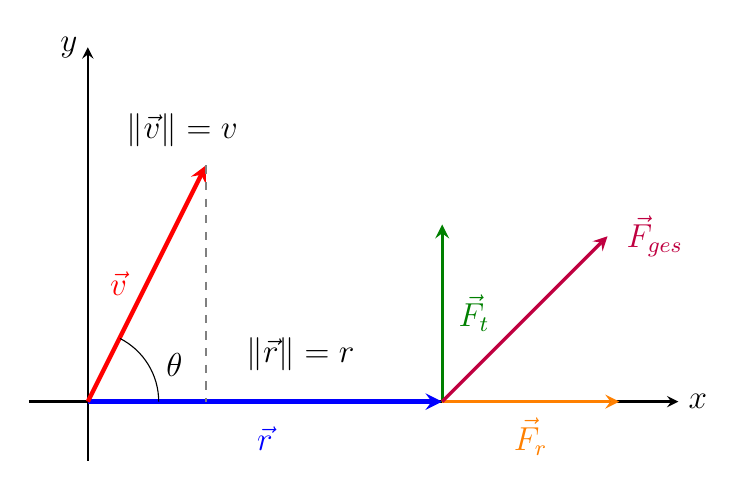
\begin{tikzpicture}[>=stealth,scale=1.5,font=\large]
% Koordinatensystem
\draw[->,thick] (-0.5,0) -- (5,0) node[right]{$x$};
\draw[->,thick] (0,-0.5) -- (0,3) node[left]{$y$};

% Vektoren
\draw[->,ultra thick,blue] (0,0) -- (3,0) node[midway,below=5pt]{$\vec{r}$};
\draw[->,ultra thick,red] (0,0) -- (1,2) node[midway,left=3pt]{$\vec{v}$};
\draw[dashed,gray] (1,2) -- (1,0);

% Kraftkomponenten
\draw[->,very thick,green!50!black] (3,0) -- (3,1.5) node[midway,right=2pt]{$\vec{F}_t$};
\draw[->,very thick,orange] (3,0) -- (4.5,0) node[midway,below=2pt]{$\vec{F}_r$};
\draw[->,very thick,purple] (3,0) -- (4.4,1.4) node[right=3pt]{$\vec{F}_{\text{ges}}$};

% Winkel
\draw (0.6,0) arc (0:63:0.6) node[midway,right=3pt]{$\theta$};
\node at (1.8,0.4) {$\|\vec{r}\| = r$};
\node at (0.8,2.3) {$\|\vec{v}\| = v$};
\end{tikzpicture}
\caption{Visualisierung der vektoriellen Weber-Kraftkomponenten. \\
$\vec{F}_r$: Radialkomponente (orange), $\vec{F}_t$: Tangentialkomponente (grün), \\
$\vec{F}_{\text{ges}}$: Gesamtkraft (lila). Die Grafik zeigt den Fall $\theta = 63^\circ$.}
\label{fig:weber_force}
\end{figure}

\subsection{Vektorielle Komponentenzerlegung}
Ausgehend von Abb.~\ref{fig:weber_force} ergeben sich die Komponenten:

\begin{align}
\vec{F}_r &= \frac{q_1 q_2}{4\pi\epsilon_0 r^2}\left[1 - \frac{v^2}{c^2} + \frac{2r a_r}{c^2}\right]\hat{r} \\
\vec{F}_t &= \frac{q_1 q_2}{4\pi\epsilon_0 r^2}\left[\frac{2v_r v_t}{c^2}\right]\hat{t}
\end{align}

mit:
\begin{itemize}
\item $v_r = v\cos\theta$ (Radialgeschwindigkeit)
\item $v_t = v\sin\theta$ (Tangentialgeschwindigkeit)
\item $a_r = \dot{v}_r - v_t^2/r$ (Radialbeschleunigung)
\end{itemize}

\subsection{Praktische Anwendungsfälle}

\textbf{Fall 1: Rein radiale Bewegung ($\theta = 0^\circ$)}
\begin{equation}
\vec{F} = \frac{q_1 q_2}{4\pi\epsilon_0 r^2}\left[1 - \frac{v^2}{c^2} + \frac{2r a}{c^2}\right]\hat{r}
\end{equation}

\textbf{Fall 2: Kreisbewegung ($\theta = 90^\circ$)}
\begin{equation}
\vec{F} = \frac{q_1 q_2}{4\pi\epsilon_0 r^2}\left[\left(1 + \frac{v^2}{c^2}\right)\hat{r} + \frac{2v^2}{c^2}\hat{t}\right]
\end{equation}
